\documentclass[12pt]{article}

\title{Virtual Synthesizer Development in C++}
\date{May 27th, 2024}

% author hijacking is so real https://tex.stackexchange.com/questions/63384/add-additional-text-on-title-page
\author{\parbox{\linewidth}{\centering%
	Will Sieber
	\endgraf\bigskip
	Department of Computer Science, The College of Wooster
	\bigskip
}}

\usepackage[left=1in,right=1in,top=1in,bottom=1in]{geometry}
\usepackage{amsmath}
\usepackage{hyperref}
\usepackage{setspace}
\usepackage{tikz-cd}
\usepackage{pgfplots}
\usepackage{graphicx}
\usepackage{listings}

\graphicspath{ {./images/} }

\spacing{1.5}

\begin{document}
\maketitle

% Latex can automatically build a table of contents for you
\newpage
\tableofcontents

\section{Abstract}
Virtual synthesizers are tools used by musicians to generate sound for use in digital audio workstations. They are repackaged dynamic-link libraries under one of several existing specifications that ensure they are compatible with host applications. Several software development kits and libraries exist with the purpose of developing these tools, but this paper will focus on development under Steinberg's Virtual Studio Technology (VST3) specification. This will serve as a quick-start guide to those interested in real time audio processing by first providing the theory behind computer audio, and then using this knowledge in a practical setting by developing a virtual additive synthesizer under the VST3 specification. This synthesizer will be able to generate several different waveforms with two different oscillators, alongside an envelope generator to control the articulation of the resulting waveform. Additional functionality common to other synthesizers will be included and discussed, but are not required to develop a functional program.
\newpage

\section{Introduction}

\subsection{Project Goals}
This project initially had one goal in mind: create sound. In order to do so, one must first process MIDI data, generate the desired waveform, and then create the user interface while ensuring the program's state changes accordingly. Upon overcoming this hurdle, several additional features could be implemented on this foundation that include additional oscillators, envelope generators, and more. Maintaining good practice while coding was an additional goal, so that others may take this project and change or modify it to their needs. That being said, prior to beginning development, it is important to understand how each element of a synthesizer works and how each fits together. 

\section{Synthesizer Basics}

\subsection{What is a Synthesizer?}
In essence, a synthesizer is a musical instrument that generates waveforms and provides several parameters to alter them in interesting ways. These parameters can interact with one another to create complex timbres, such as by introducing additional frequencies to a sound.

\subsection{Components}
There are several components of a synthesizer that work together in order to generate sound. This section will cover in detail the specific components that were implemented in software. Following this section, there will be another that provides further components that are commonly found in other synthesizers.

\subsubsection{Oscillators}
Oscillators can be generally broken into two categories: tone generators and controllers. Tone generators repeat periodic waves in order to generate sound. Simple tone generators can be expressed as mathematical expressions, such as \(f(x) = sin(x)\), while complex tone generators allow for any waveform to be repeated, regardless if they can be easily expressed as a single expression. Complex oscillators generally allow for a number of different waveforms to be represented in a single table, allowing for a user to select any number of waveforms in real time. For the purposes of this project, simple oscillators are used as tone generators. Controller oscillators, on the other hand, are much lower frequency than tone oscillators, and are used to control other parameters of a synthesizer. These will be discussed in brief at a later section.

There are four simple waveforms that are considered "fundamental" for a synthesizer. These are the oscillator's \textit{sine}, \textit{square}, \textit{sawtooth}, and \textit{triangle} waveforms. Each have their own characteristics distinguishing them from one another, but can be loosely described in the following ways:

\begin{enumerate}
	\item Sine waves are considered "pure", as they contain no overtones. Should every instrument be isolated to its fundamental frequency, this is the tone that would result.
	\item Square waves are "buzzy" and [].
	\item Sawtooth waves are [].
	\item Triangle waves are [].
\end{enumerate}

\subsubsection{Envelope Generators}
In order to provide articulation, envelope generators describe how the amplitude of a particular sound should change over time. Several parameters are used to accomplish this goal, and those are the synthesizer's \textit{attack}, \textit{decay}, \textit{sustain}, and \textit{release}. \textit{Attack} describes how much time it takes for the synthesizer to reach full amplitude upon receiving the signal to generate sound. Note that this is not the s A short attack will reach full amplitude quickly, such as playing on a piano or organ. Longer attacks will take more time to reach full amplitude, which create a "swelling" effect that is similar to that of a violin increasing in volume. \textit{Decay} describes how much time the synthesizer should take to reach a particular amplitude once the attack is finished. A longer decay will prolong a sound prior to the sustain, and vice versa. \textit{Sustain}, unlike attack and decay, describes the amplitude itself to which the decay will reach upon completion. When reached, the synthesizer will continuously play at this amplitude until a signal is sent that it should stop generating sound. Upon this signal, \textit{release} describes how long the synthesizer should take to stop generating sound by gradually decreasing the amplitude to zero. 

In more technical terms, the envelope generator of our synthesizer is its own finite state machine that modifies our signal. The signal is modified by multiplying our source to a constantly changing value. This value has different behavior as to how it changes depending on if it is in the attack state, the decay state, and so on.  

One may notice a problem with this model - the rate at which the attack, decay, and release change amplitude itself is not described. Powerful synthesizers allow for this change to be represented as a polynomial function, but for the purposes of this project, the rate at which each parameter changes will simply be linear. 

With these two components in mind, one can create a simple synthesizer in the same manner that is described in this project. What follows are additional components found commonly in synthesizers, but are not required to be present. That being said, it is important to understand them to provide a complete picture of what synthesizers are capable of. 

\subsection{Extra Components}

\subsubsection*{Digitally Controlled Amplifiers}
Digitally Controlled Amplifiers (DCAs) control the final amplitude or volume of the synthesizer. A good DCA will prevent the final output signal from going beyond the range [-1, 1] thus preventing unwanted artifacts. They can handle global panning as well, allowing the user to choose where the resulting sound should play from a pair of speakers. \cite{Pirkle_2015} For the purposes of this project, volume is controlled from each source oscillator.

\subsubsection*{Low-Frequency Oscillators}
Low-Frequency Oscillators (LFOs) are generally used as an input to automate other parameters of a synthesizer, allowing for a greater range of timbres. They generally exist in a range much lower than human hearing (\textless 20 Hz) and usually consist ofs the same basic waveforms that tone generator oscillators use (sine, square, sawtooth, and triangle).

\subsubsection*{Filters}
Filters are a form of subtractive synthesis that remove frequencies based on a particular \textit{cutoff}. There are several types of filters that exist, with the most common being \textit{lowpass}, \textit{highpass}, and \textit{bandpass}. Lowpass filters remove higher frequencies, allowing lower frequencies to "pass through" the filter, resulting in a "dark" sound. Highpass filters do the opposite, removing lower frequencies and passing through higher ones based on a particular cutoff frequency. Bandpass filters remove both upper and lower frequencies from a particular cutoff.

\subsection{Additive Synthesis}
Strictly speaking, this synthesizer will not be a fully functional additive synthesizer. By definition, an additive synthesizer works by adding sine waves of proper frequencies and amplitudes in order to generate the resulting wave one desires. \cite{Pirkle_2015} Doing so this way is considered "cleaner" and removes aliasing from the resulting wave. 

\subsection{Extra Synthesis Techniques}

\subsubsection*{Subtractive Synthesis}
Subtractive synthesis is done by taking a wave and removing frequencies from the waveform. Filters are an example of subtractive synthesis, which have been covered in a previous section. 

\subsubsection*{Wavetable Synthesis}
Wavetable synthesis is a type of synthesis that allows a musicians to manipulate the waveform being used in real time. Instead of there being one of several simple waveforms to choose from, the user can select an entire array (or table) of waveforms that can be morphed from one to the next. This is known as \textit{digital interpolation}. 

\subsubsection*{FM Synthesis}
Frequency modulation (FM synthesis) is a type of waveform manipulation that uses one waveform to manipulate the frequency of another. An example of this can be see below: 


\section{Implementation}

\subsection{Theory}
There are a number of problems one faces when attempting to process real time audio. They can be summed up by asking the following questions:

\begin{enumerate}
	\item "How do we create a digital representation of sound?"
	\item "How do we process audio fast enough to ensure there are no unwanted artifacts in our software?"
\end{enumerate}

The following section will address these concerns and provide the theory of what is occurring in the background of our software.

\subsubsection{Discrete Signals}
Sound is represented digitally by taking samples of the original source. An audio sample measures the amplitude of the source wave at a point in time, which is represented in code as a floating point number in the range \([-1, 1]\). Given a piece of audio, the number of samples per second represent the \textit{sample rate} of our recording. As a result, a higher sample rate will result in audio that more closely resembles the original source. Consider the following sine wave:

\begin{figure}[h] % [h] used to prevent {figure} from doing weird positioning
\begin{center}
	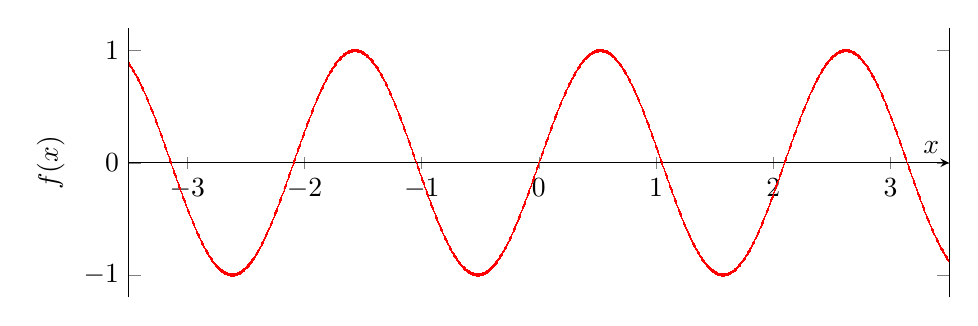
\begin{tikzpicture}
		\begin{axis} [
			axis x line = middle, % The x axis should go through the origin
			xlabel = \(x\),
			ylabel = {\(f(x)\)},
			height = 5cm,
			width = 12cm
			]
			
			\addplot [
			jump mark mid,
			domain = -3.5:3.5,
			samples = 1000,
			very thick, red
			] {(sin(deg(3 * x)))};
			
		\end{axis}
	\end{tikzpicture}
	\caption{A graph of the sine wave \(f(x) = sin(3x)\).}
\end{center}
\end{figure}

A computer would interpret this signal by taking a number of samples at regular intervals:

\begin{figure}[h] % [h] used to prevent {figure} from doing weird positioning
	\begin{center}
		\begin{tikzpicture}
			\begin{axis} [
				axis x line = middle, % The x axis should go through the origin
				xlabel = \(x\),
				ylabel = {\(f(x)\)},
				height = 5cm,
				width = 12cm
				]
				
				\addplot+ [
				ycomb,
				mark = text,
				text mark = , % so jank
				domain = -3.5:3.5,
				samples = 40,
				red
				] {(sin(deg(3 * x)))};
				
			\end{axis}
		\end{tikzpicture}
		\caption{A discrete graph of the sine wave \(f(x) = sin(3x)\) taken with 40 samples.}
	\end{center}
\end{figure}

Thus, the higher number of samples per second would result in a sound that more closely resembles Figure 1:

\begin{figure}[h] % [h] used to prevent {figure} from doing weird positioning
	\begin{center}
		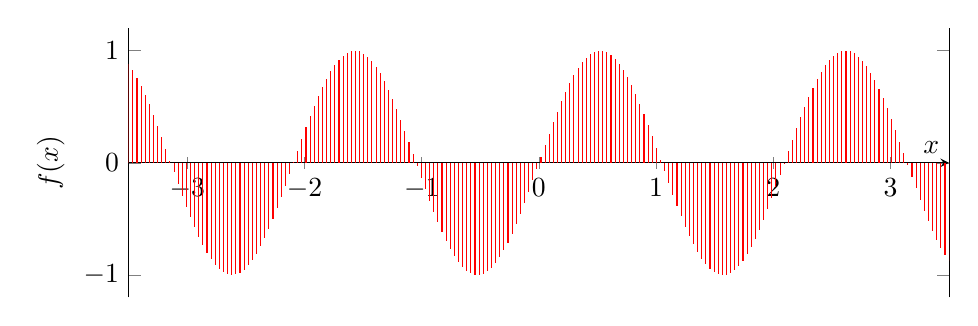
\begin{tikzpicture}
			\begin{axis} [
				axis x line = middle, % The x axis should go through the origin
				xlabel = \(x\),
				ylabel = {\(f(x)\)},
				height = 5cm,
				width = 12cm
				]
				
				\addplot+ [
				ycomb,
				mark = text,
				text mark = , % so jank
				domain = -3.5:3.5,
				samples = 200,
				red
				] {(sin(deg(3 * x)))};
				
			\end{axis}
		\end{tikzpicture}
		\caption{A discrete graph of the sine wave \(f(x) = sin(3x)\) taken with 200 samples.}
	\end{center}
\end{figure}


Most commonly, audio files will have a sample rate of 44.1 kHz or 48 kHz. That means our software will need to process that number of samples per second, continuously. For the purposes of this project, there are two audio sources: \textit{OSC1} and \textit{OSC2}. Each oscillator will generate a sound sampled at the rate that is decided by the host application.

\subsubsection{Buffers}
To process this large amount of data quickly, \textit{buffers} are used.

\subsubsection{Flow of Information}

% the goat https://ctan.math.washington.edu/tex-archive/graphics/pgf/contrib/tikz-cd/tikz-cd-doc.pdf
% i am just gonna put an image here
\begin{center}
	\begin{figure}[h]
		\includegraphics[scale=0.4]{image1.png}
		\caption{A graph of how audio information is handled throughout the system.}
	\end{figure}
\end{center}

\subsection{Comparison of Frameworks}
There are several competing standards to create virtual synthesizers (among other pieces of music software). They include - but are not limited to - VST(3), AU, AAX (DSP/Native), LV2, and CLAP. Each have their own benefits and drawbacks, but can largely be broken down into "what operating system are you writing for". VST is supported on both Windows and MacOS, while AU and AAX are supported exclusively on MacOS. 

\subsection{Development with VST3 SDK}


\subsubsection{Development Tools}
The VST3 SDK contains several tools and programs that assist in developing the boilerplate code necessary for creating VST applications and ensuring they fall under the required specification. These are the project generator, GUI editor, and validator. By using the project generator, a CMakeLists text file is generated. The program automatically compiles it, which creates a Visual Studio solution pre-configured with several components to test VST applications easily. 

When the Visual Studio solution is started, a host application is started that can be used to quickly test MIDI input and audio output.

\subsubsection{Workflow and UML diagram}
Functions and classes under the VST3 SDK are organized under namespaces, in order to avoid name collisions \cite{Pirkle_2015}. The Steinberg namespace contains the Vst namespace, which in turn contains the programmer's namespace created by the project generator. 

\subsection{Creating Oscillators}
There are several methods of generating sine, square, saw, and triangle waves. 

\subsection{Creating An Envelope Generator}

\section{Conclusion and Future Work}


% Bibliography
\bibliography{bibliography}
\bibliographystyle{abbrv}

\end{document}